\documentclass[12pt,a4paper,oneside]{book}
\usepackage[utf8]{inputenc}
\usepackage[spanish]{babel}
\usepackage[T1]{fontenc}
\usepackage{textcomp}
\usepackage[T1]{fontenc}
\usepackage{hyperref}
\usepackage{amsmath}
\usepackage{amsfonts}

\usepackage{amssymb}
\usepackage{graphicx}
\usepackage[utf8]{inputenc}
\usepackage[left=2.54cm, right=2.54cm, top=2.54cm, bottom=2.54cm]{geometry}
\usepackage{tabularx}
\usepackage{listings}[utf8]
\usepackage{xcolor}
\usepackage{makeidx}
\raggedbottom
\makeindex
\date{\today}

\hypersetup{
	colorlinks=true,
	linkcolor=blue,
	filecolor=magenta,
	urlcolor=cyan,
	pdftitle={Overleaft Example},
}

\definecolor{codegreen}{rgb}{0,0.6,0}
\definecolor{codegray}{rgb}{0.5,0.5,0.5}
\definecolor{codepurple}{rgb}{0.58,0,0.82}
\definecolor{backcolour}{rgb}{0.95,0.95,0.92}

\lstdefinestyle{mystyle}{
	backgroundcolor=\color{backcolour},   
	commentstyle=\color{codegreen},
	keywordstyle=\color{blue},
	numberstyle=\tiny\color{codegray},
	stringstyle=\color{codepurple},
	basicstyle=\ttfamily\footnotesize,
	breakatwhitespace=false,         
	breaklines=true,                 
	captionpos=b,
	keepspaces=true,                 
	numbers=left,                    
	numbersep=5pt,                  
	showspaces=false,                
	showstringspaces=false,
	showtabs=false,                  
	tabsize=4,
	classoffset=1,% starting a new class
	morekeywords={True},
	keywordstyle=\color{red},
	classoffset=6,% starting a new class
	morekeywords={True},
	keywordstyle=\color{green},
	classoffset=0,
}

\usepackage{caption}
\captionsetup[table]{name=Tabla}
\renewcommand*{\lstlistingname}{Exemplo de código}
\renewcommand{\listfigurename}{Figuras}
\renewcommand{\listtablename}{Tablas}

\pagenumbering{arabic}
\lstset{
	style=mystyle,
	inputencoding=utf8,
	extendedchars=true,                    
	literate={á}{{\'a}}1 {ã}{{\~a}}1 {é}{{\'e}}1,
}

%Final Python listing configuration
% Biliografia configuracion
\usepackage[
backend=biber,
style=alphabetic,
sortcites,
url=true
]{biblatex}
\addbibresource{bibliography.bib}
\captionsetup[figure]{labelformat=simple,justification=centerlast}

\begin{document}
	\begin{titlepage}
	\noindent
	\centering
	\Large {SOFTWARE DEVELOPMENT PLANNING}
	\begin{center}
		\centering
		\rule{150 mm}{0.1 mm}
		\Large {AGILE JIRA\\}
		
		\rule{150 mm}{0.1 mm}
		\large {{Software Development Planning con Jira y Agile para Organizar y Gestionar el Desarrollo de Software}}
		\rule{150 mm}{0.4 mm}
		\vspace{1 cm}
		\vspace{0.3 cm}
		
\includegraphics[width=1\textwidth]{image/cover.jpg}
	\end{center}
	\vspace{0.3 cm}
	\begin{center}
		{\large AUTOR
			{\href{https://github.com/titoroopart}{@TITOR-OOPART}}}	\\
		{\large YOUTUBE:	{\href{https://www.youtube.com/@ReadToRun}{@ReadToRun}}}	\\
		{\large GITHUB BOOK:  	{\href{https://github.com/titoroopart/SoftwareDevelopmentPlanning_book#}{@SoftwareDevelopmentPlanning\_book}}}\\
	\end{center}
	\vspace{0.5 cm}
	\vfill
	\begin{center}
		\large\today
	\end{center}
\end{titlepage}

	\thispagestyle{empty}
	\tableofcontents
	\listoffigures
	\listoftables
	\lstlistoflistings
	\chapter{Introducción Planeamiento (Plan01)}
El planeamiento del desarrollo de software es uno de los proceso mas importante a la hora de desarrollar un proyecto de software.
Un buen planeamiento (Planning) nos permitirá tener un idea solida de todo los puntos que nos encontraremos en el proyecto como por ejemplo.
\begin{enumerate}
  \item Definir el Alcance (Scope) - Aquí se deja en claro todo lo que se desarrollara en un tiempo definido y se especifica que cosas son descartadas 
  \item Crear y Priorizar Tareas - Divide el proyecto en tareas manejables y se les da prioridad para su ejecución.
  \item Anticiparse a Problemas - Identifica riesgos y busca soluciones.
  \item Estimación de Tiempo y Recursos - Calcula tiempo y la persona a cargo de cada tarea.
  \item Elegir Tecnologías y Arquitectura - Define la estructura y las tecnologías que serán usadas.
  \item Plan de Pruebas (Testing) - Asegura la calidad antes del lanzamiento.
  \item Plan de Comunicación y Entregables - Coordina al equipo y forma de manejar los artifacts (entregables)
\end{enumerate}
\section{Agile y Scrum}
Un método muy popular para el planeamiento en el mundo de desarrollo de software es usar la metodología de trabajo Agile(Ágil) + Scrum puedes revisar SCURM.ORG para mantenerte al día.
\\
El principio Scrum es un proceso control del proyecto con(Transparencia, inspección y adaptación)  colaborativa basado en priorizar tareas.
Para llevar a cabo una reunión de Scrum deben estar presentes todos los miembros del equipo aunque en algunas ocasiones puede faltar alguno \cite{104049401}.

\begin{enumerate}
  \item Product Owner (PO) - Decide qué features se construyen.
  \item  Scrum Master (SM) - Elimina obstáculos y asegura que Scrum se siga correctamente.
  \item Equipo de Desarrollo (Developers + Testers) - Deciden cómo implementar las tareas (técnicamente).
\end{enumerate}
\begin{center}
	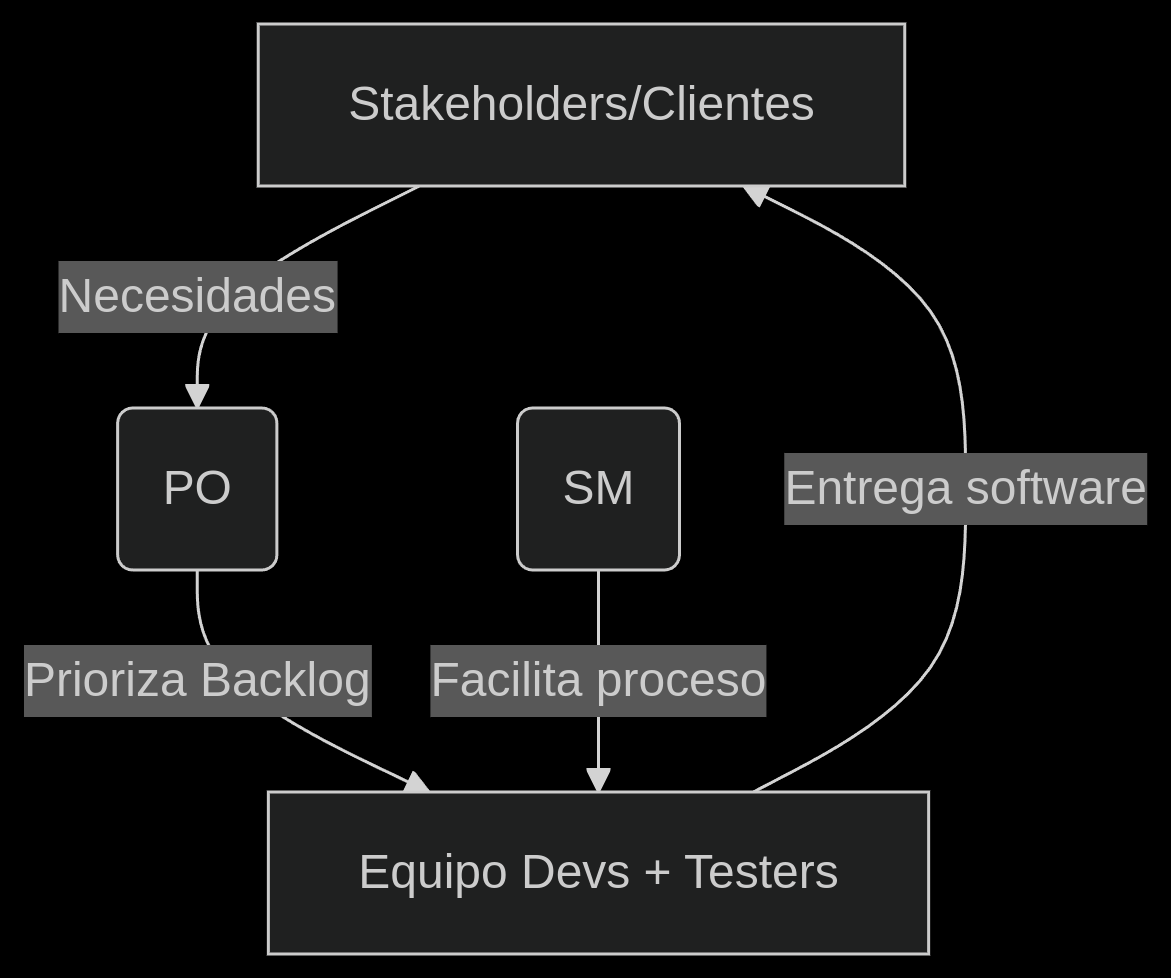
\includegraphics[width=0.7\textwidth]{image/scrum_team.png}
\end{center}

En este proceso tenemos dos eventos que son muy importantes que son el backlog, sprint y board.
\begin{enumerate}
  \item Backlog - Sección donde se escribirán todas las tareas en las que trabajara para el siguiente lanzamiento.
  \item Sprint - Tiempo de 2-4 semanas donde se trabajan tareas seleccionadas del backlog.
  \item Board - Lugar donde se ve el estado de las tareas del sprint tiene comunmente 4 secciones.
    \begin{enumerate}
      \item To Do - Tareas que todavía no se iniciaron ni asignaron.
      \item Doing o In progress - Tareas que estas siendo desarrolladas.
      \item Testing - Lugar donde se verifica que las tareas completadas cumplen con el aceptance criteria.
      \item Done - Lugar para tareas completadas que pasaron las pruebas de calidad.
    \end{enumerate}
\end{enumerate}

\section{Jira}
Jira es una herramienta de gestión de proyectos y seguimiento de errores desarrollada por Atlassian. Es ampliamente usada en las empresas para desarrollar proyectos de software.\\
En Jira tenemos implementadas varias plantillas listas para ser usadas entre ellas la metodología Ágil Scrum.
\\
\subsection{Backlog}
En Jira tenemos contamos con un backlog explicado anteriormente donde podremos crear  diferentes tareas se marcara con * las que son obligatorias.
\begin{enumerate}
  \item Epic - Funcionalidad grande que puede ser dividida en tareas mas pequeñas(Un Epic llega a ser el objetivo general del equipo)
  \item Story - Tarea que es llevada a cabo en el transcurso del sprint esta cuenta de diferentes partes.
    \begin{enumerate}
      \item *Titulo - Titulo descriptivo de la tarea
      \item *Descripción - resumen de lo que se trabajara
      \item *Acceptance criteria - Criterio de aceptación, o requisitos para que se considere tarea terminada.
      \item *Prioridad - Urgencia de la tarea.
      \item *Story Point - Estimación de esfuerzo (1,2,3,5,8,13) debe seguir la sucesión fibonacci
      \item *Labels - Etiqueta para ver a donde pertenece (frontend, backend, api, etc)
      \item Attachments - Documentos screenshots si es necesario
    \end{enumerate}
  \item Bug - Bug error de programación encontrado en el software
    \begin{enumerate}
      \item *Titulo - Titulo descriptivo del bug.
      \item *Descripción - Descripción del error y los pasos para reproducir el error y ambiente donde fue encontrado versión etc.
      \item *Severidad - Impacto en el software del bug Blocker, Critical, Major, Minor(Valor determinado por el Tester).
      \item *Prioridad - Que tan rápido debe ser fixeado(Valor determinado por el PO).
      \item Attachments - Documentos screenshots video si es necesario.
    \end{enumerate}
  \item Task - Un Task (Tarea) en Jira se usa para trabajos concretos que no son bugs ni historias de usuario (configuraciones, investigaciones, tareas técnicas)
\end{enumerate}
\subsection{Board}
Lugar donde podemos ver los tickets del sprint comúnmente se tiene 3 secciones To do, Doing o In Progress, Done pero en los proyectos se les suele aumentar Testing  o In Review para las pruebas de calidad.
\begin{center}
	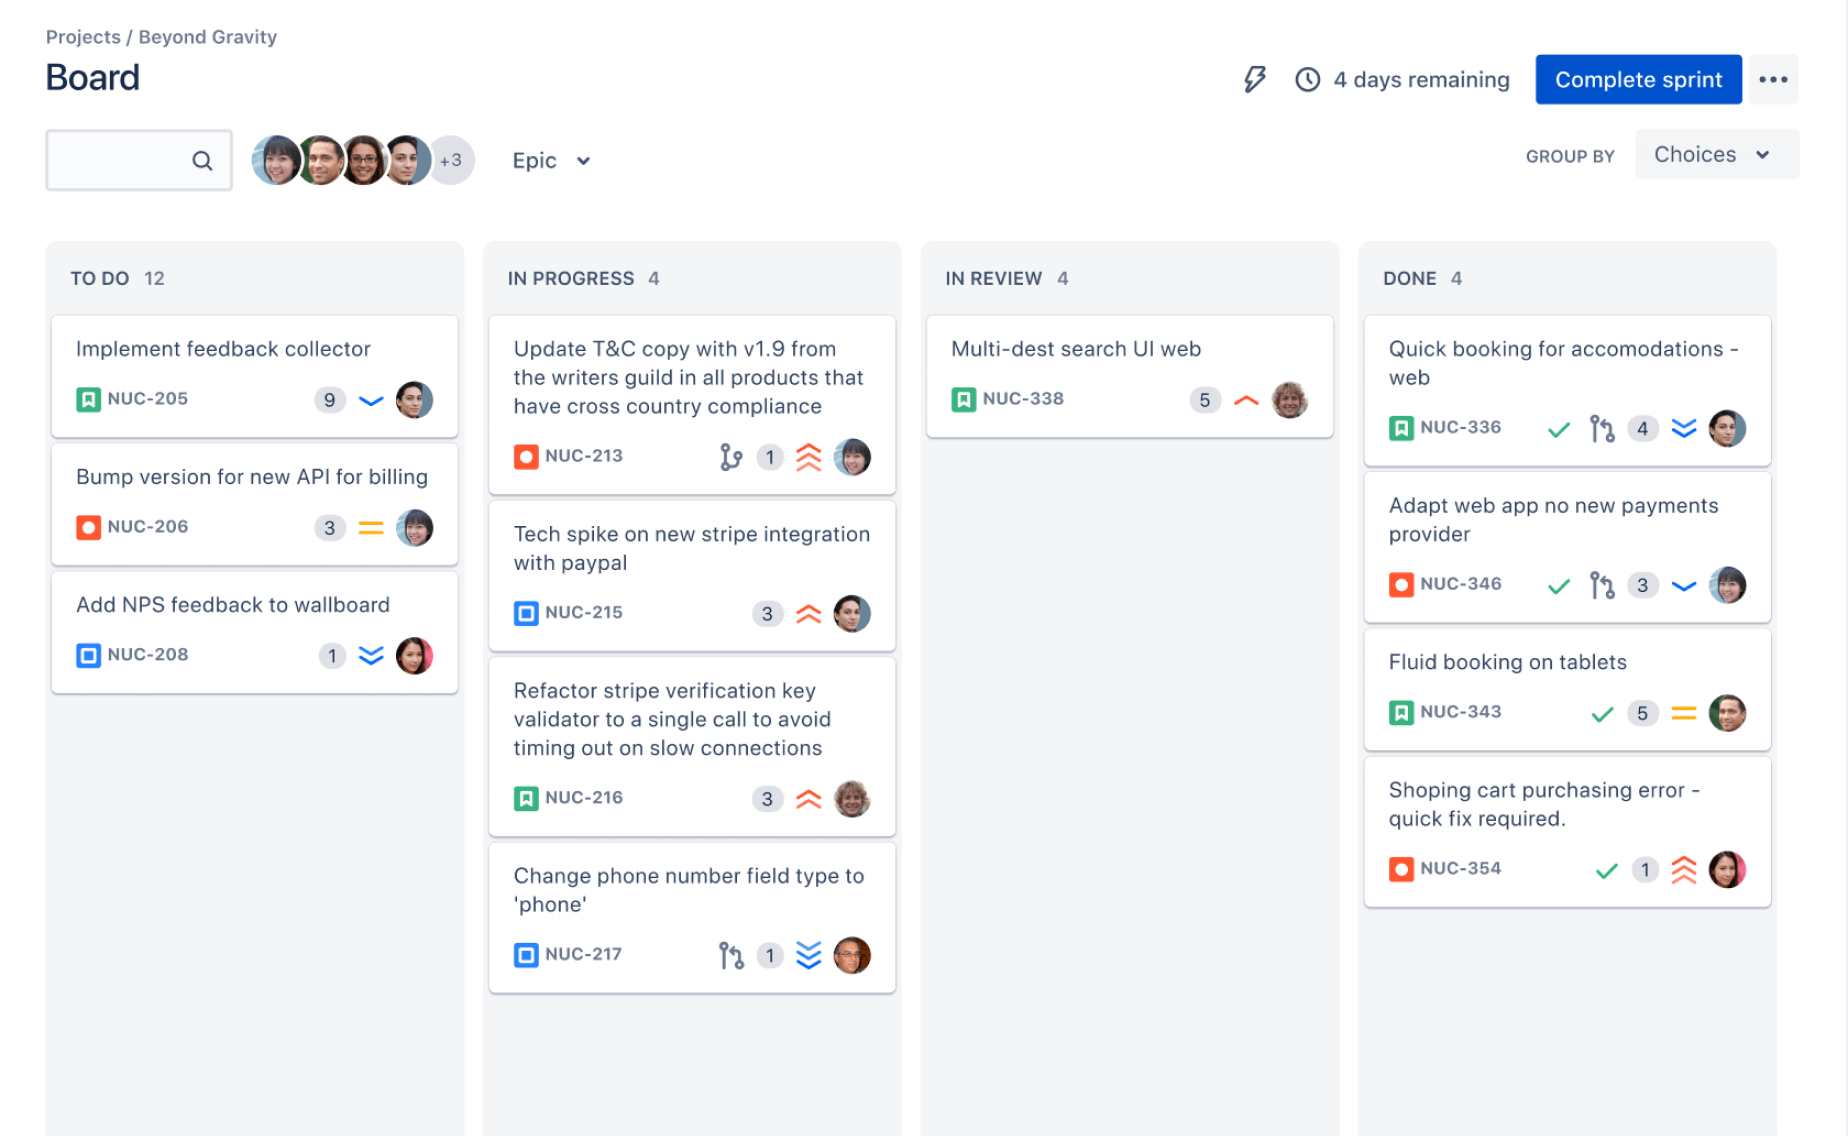
\includegraphics[width=1\textwidth]{image/scrum-board.png}
\end{center}








	\printbibliography[heading=bibintoc]
\end{document}
